\documentclass{article}
\usepackage[utf8]{inputenc}
\usepackage[icelandic]{babel}
\usepackage[T1]{fontenc}
\usepackage{graphicx}
\usepackage{mathtools}
\usepackage{amsmath}
\usepackage{amssymb}
\usepackage{minted}
\usepackage{listings}
\usepackage{color}

\definecolor{dkgreen}{rgb}{0,0.6,0}
\definecolor{gray}{rgb}{0.5,0.5,0.5}
\definecolor{mauve}{rgb}{0.58,0,0.82}

\lstset{frame=tb,
  language=Java,
  aboveskip=3mm,
  belowskip=3mm,
  showstringspaces=false,
  columns=flexible,
  basicstyle={\small\ttfamily},
  numbers=none,
  numberstyle=\tiny\color{gray},
  keywordstyle=\color{blue},
  commentstyle=\color{dkgreen},
  stringstyle=\color{mauve},
  breaklines=true,
  breakatwhitespace=true,
  tabsize=3
}


\graphicspath{ {./imgs} }
\title{v3 - Tölv 2}
\author{ttb3@hi.is}
\date{\today}

\begin{document}
\maketitle


\section*{Dæmi 2}

\begin{lstlisting}
    public static void skilarRod(int[] a, int[] b) {
            int n = (a.length + b.length) ;
            int indexA = 0;
            int indexB = 0;
    
            boolean aBuid = false;
            boolean bBuid = false;
    
            String out = "";
    
            for (int i = 0; i < n; i++) {
                
                if ((!aBuid && a[indexA] < b[indexB]) || bBuid) {
                    if (indexA == a.length-1) aBuid = true;
                    out += Integer.toString(a[indexA])+", ";
                    if (indexA < a.length-1) indexA++;
                }
    
                else {
                    if (indexB == b.length-1) bBuid = true;
                    out += Integer.toString(b[indexB])+", ";
                    if (indexB < b.length-1) indexB++;
                }
            }
            
            System.out.println(out);
        }
\end{lstlisting}

\section*{Dæmi 3}
\begin{center}
    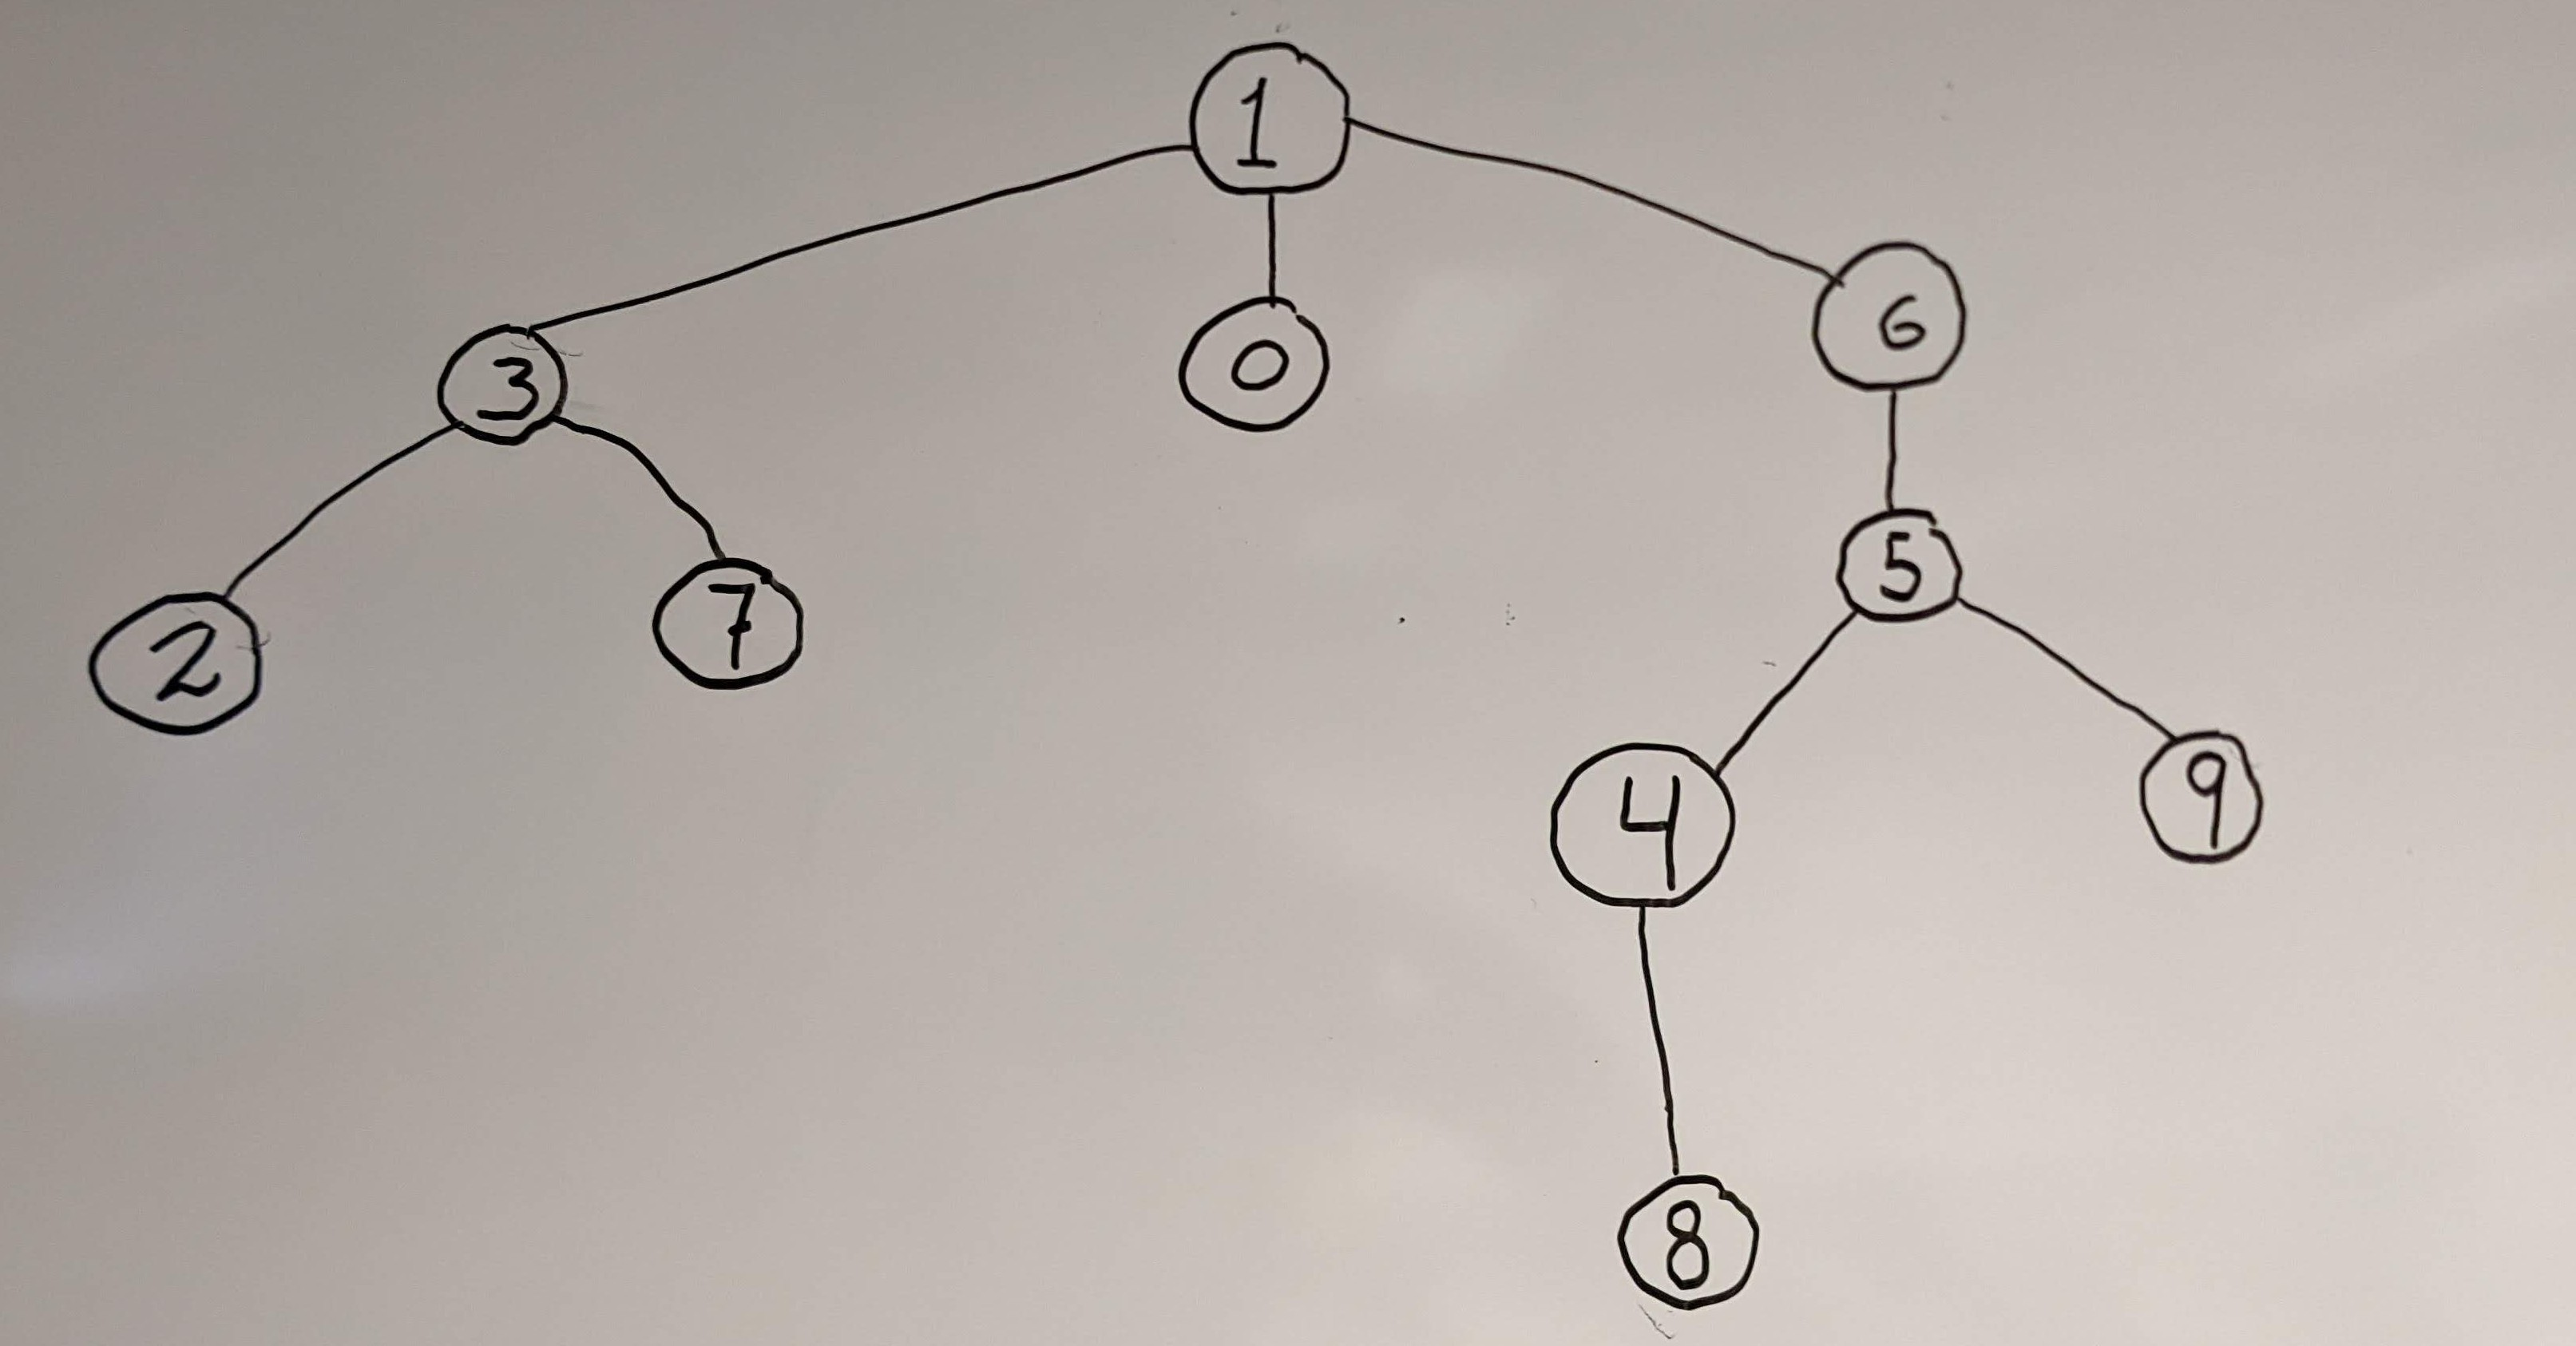
\includegraphics[scale=0.1]{imgs/tree_159.jpg}
\end{center}


\end{document}